\documentclass{labreport}

\begin{document}

\labtitle
    {5}
    {Empirical Analysis of Greedy Algorithms for Minimum Spanning Trees: Prim vs Kruskal}
    {Student}
    {Covali Ilie, st. gr. FAF-243}
    {asist. univ. Fistic Cristofor}

\tableofcontents
\newpage

\lstset{style=python}

\section{Algorithm Analysis}

\subsection{Objective}

Implement and evaluate two classical greedy methods for minimum spanning trees, Prim and Kruskal, then compare their practical behavior across graph sizes and density regimes.

\subsection{Tasks}

\begin{enumerate}
    \item Implement Prim's algorithm and Kruskal's algorithm in a programming language.
    \item Design test graphs of varying sizes and densities (sparse and dense).
    \item Establish appropriate metrics for comparing algorithm performance, including both execution time and algorithm-specific operations.
    \item Conduct empirical analysis across a range of input sizes.
    \item Present results in tabular and visual formats with thorough analysis.
    \item Draw conclusions about algorithm selection based on graph properties.
\end{enumerate}

\subsection{Theoretical Notes}

Empirical evaluation is essential because asymptotic complexity alone does not fully predict practical performance. Constant factors, chosen data structures, and runtime environment can significantly influence measured execution time. In this report, empirical analysis is used to:

\begin{enumerate}
    \item Confirm theoretical expectations using measured data.
    \item Compare algorithms on real runtime characteristics.
    \item Expose the impact of implementation constants and overhead.
    \item Provide practical guidance for selecting an algorithm.
\end{enumerate}

The workflow follows standard methodology: define objectives, choose metrics, generate representative test data, execute repeated runs, and analyze trends in the resulting measurements.

\subsection{Introduction}

The minimum spanning tree (MST) problem is a central topic in graph theory with applications in network design, clustering, and infrastructure optimization. Given a connected, undirected, weighted graph, the objective is to connect all vertices with minimum total edge weight and no cycles.

MSTs can be solved optimally with greedy algorithms, notably Prim and Kruskal. Both are mathematically correct due to MST properties such as cut and cycle criteria, but they follow different strategies:

\begin{itemize}
    \item \textbf{Prim's algorithm} expands a single tree by repeatedly adding the minimum-weight edge from the current tree to an outside vertex.

    \item \textbf{Kruskal's algorithm} processes all edges globally in nondecreasing order and keeps an edge only if it connects two distinct components.
\end{itemize}

Although both algorithms can have similar asymptotic behavior in some regimes, their practical efficiency depends on graph density, data representation, and implementation overhead. This lab provides a direct empirical comparison.

\subsection{Comparison Metric}

The primary metric is \textbf{execution time} (milliseconds, measured with high-resolution counters). To interpret time differences, we also capture algorithm-specific counters:

\begin{itemize}
    \item \textbf{Prim:} key updates (priority queue relaxations), edges considered, and heap operations.
    \item \textbf{Kruskal:} edges examined, edges accepted into MST, and union-find operations.
    \item \textbf{Both:} peak memory usage (KiB) and observed growth slopes from log-log regression.
\end{itemize}

These metrics show not only which algorithm is faster, but also the reason behind the difference.

\subsection{Input Format}

Each algorithm is tested on increasing graph sizes under two density regimes:

\begin{itemize}
    \item \textbf{Sparse graphs:} nodes $n \in \{10, 20, 30, 50, 75, 100, 150, 200, 300, 400, 500\}$, average degree about 4, so $E \approx 2n$.

    \item \textbf{Dense graphs:} nodes $n \in \{10, 20, 30, 50, 75, 100, 150, 200, 250, 300, 350\}$, edge probability 0.65, so $E \approx 0.325n^2$.
\end{itemize}

All instances are undirected and weighted with random integers from 1 to 100. Each setup is repeated 3 times, and reported values use averages and ranges. Random seeds are fixed by graph size for reproducibility.

\section{Implementation}

All algorithms are implemented in Python with emphasis on correctness and readability. The objective is empirical comparison rather than low-level micro-optimization.

\subsection{Prim's Algorithm}

Prim builds the MST incrementally from an initial vertex (vertex 0 in this implementation). It tracks vertices already included and uses a priority queue of candidate edges connecting inside to outside vertices.

\textbf{High-level approach:}
\begin{enumerate}
    \item Initialize with a starting vertex; mark it as part of MST.
    \item Repeat until all vertices are included:
    \begin{enumerate}
        \item Select the minimum-weight edge crossing from MST to non-MST.
        \item Add that edge and the new vertex to MST.
    \end{enumerate}
\end{enumerate}

\textbf{Complexity analysis:}

The complexity depends on the chosen priority-queue strategy. With a binary heap:
\begin{align*}
    T(V, E) = O((V + E) \log V)
\end{align*}

For sparse graphs with $E \approx V$, this is near $O(V \log V)$. For dense graphs with $E \approx V^2$, it becomes near $O(V^2 \log V)$.

A matrix-based Prim variant with linear minimum selection gives $O(V^2)$ and can be preferable on dense inputs where heap overhead is expensive.

\textbf{Key Metrics:} The algorithm's work is measured by key updates (priority queue insertions/relaxations), edges considered from the adjacency list, and heap operations performed.

\textbf{Data structures:} Prim uses an adjacency list representation for sparse graphs (to avoid examining non-existent edges) and an adjacency matrix representation for dense graphs (to avoid heap overhead when all pairs need consideration).

\textbf{Key technique:} For the heap-based variant, a binary min-heap maintains candidate edges. When a vertex is added to the MST, all its incident edges are considered and inserted or updated in the heap.

\textbf{Pseudocode:}
\begin{lstlisting}[language=Python]
def prims_algorithm(n, adj_list):
    in_mst = [False] * n
    heap = [(0.0, 0, -1)]  # (weight, node, parent)
    mst_edges = []

    while heap:
        weight, u, parent = heappop(heap)
        if in_mst[u]:
            continue
        in_mst[u] = True

        if parent != -1:
            mst_edges.append((parent, u, weight))

        for v, w in adj_list[u]:
            if not in_mst[v]:
                heappush(heap, (w, v, u))

    return mst_edges
\end{lstlisting}

\subsection{Kruskal's Algorithm}

Kruskal constructs the MST by scanning edges globally in nondecreasing weight order and accepting only those edges that do not create cycles.

\textbf{Description:} All edges are sorted by weight. The algorithm then traverses this sorted list; if an edge links two different components (checked with union-find), it is added to the MST and the components are merged. The process stops after selecting $V - 1$ edges.

\textbf{Complexity Analysis:}
Sorting dominates the complexity: $O(E \log E)$ for sorting, plus $O(E \alpha(V))$ for union-find operations, where $\alpha(V)$ is the inverse Ackermann function (effectively constant). This yields near $O(V \log V)$ in sparse regimes and near $O(V^2 \log V)$ in dense regimes.

\textbf{Key Metrics:} The algorithm's work is measured by edges examined, edges selected for the MST, and union-find operations performed.

\textbf{Data structures:} Kruskal uses an edge list and a union-find data structure. The union-find maintains which vertices belong to which connected component, enabling efficient cycle detection.

\textbf{Key technique:} Edges are sorted by weight once. Then, the algorithm iterates through edges; if the endpoints are in different components (determined by union-find), the edge is added to the MST and components are merged.

\textbf{Pseudocode:}
\begin{lstlisting}[language=Python]
def kruskal_algorithm(n, edges):
    mst_edges = []
    sorted_edges = sorted(edges, key=lambda x: x[2])
    uf = UnionFind(n)

    for u, v, w in sorted_edges:
        if uf.union(u, v):  # Different components
            mst_edges.append((u, v, w))
            if len(mst_edges) == n - 1:
                break

    return mst_edges
\end{lstlisting}

\subsection{Union-Find Implementation}

The union-find structure applies path compression and union by rank, making operations nearly constant amortized time.

\textbf{Pseudocode:}
\begin{lstlisting}[language=Python]
class UnionFind:
    def __init__(self, n):
        self.parent = list(range(n))
        self.rank = [0] * n

    def find(self, x):
        if self.parent[x] != x:
            self.parent[x] = self.find(self.parent[x])
        return self.parent[x]

    def union(self, x, y):
        root_x, root_y = self.find(x), self.find(y)
        if root_x == root_y:
            return False
        if self.rank[root_x] < self.rank[root_y]:
            self.parent[root_x] = root_y
        else:
            self.parent[root_y] = root_x
            if self.rank[root_x] == self.rank[root_y]:
                self.rank[root_x] += 1
        return True
\end{lstlisting}

\section{Empirical Results and Analysis}

\subsection{Sparse Graphs: Results and Analysis}

\begin{table}[H]
    \centering
    \small
    \begin{tabular}{|c|c|c|c|c|}
    \hline
    \textbf{n} & \textbf{m} & \textbf{Prim (ms)} & \textbf{Kruskal (ms)} & \textbf{Speedup} \\
    \hline
     10 &    21 &   0.052 &   0.069 &  1.32x \\
     20 &    35 &   0.069 &   0.053 &  0.76x \\
     30 &    57 &   0.105 &   0.068 &  0.65x \\
     50 &    94 &   0.161 &   0.123 &  0.76x \\
     75 &   165 &   0.271 &   0.214 &  0.79x \\
    100 &   215 &   0.392 &   0.289 &  0.74x \\
    150 &   290 &   0.617 &   0.404 &  0.65x \\
    200 &   375 &   0.856 &   0.525 &  0.61x \\
    300 &   637 &   1.551 &   0.960 &  0.62x \\
    400 &   765 &   1.983 &   1.306 &  0.66x \\
    500 &   990 &   2.673 &   1.629 &  0.61x \\
    \hline
    \end{tabular}
    \caption{Sparse Graphs: Prim vs Kruskal Execution Time}
    \label{tab:sparse_comparison}
\end{table}

Figure~\ref{fig:sparse_time_vs_nodes} plots the sparse-regime timings from Table~\ref{tab:sparse_comparison}. Both curves increase with $n$, but Kruskal remains below Prim for nearly the full range after the smallest inputs. The widening separation indicates a stable performance pattern rather than random fluctuation.

\begin{figure}[H]
    \centering
    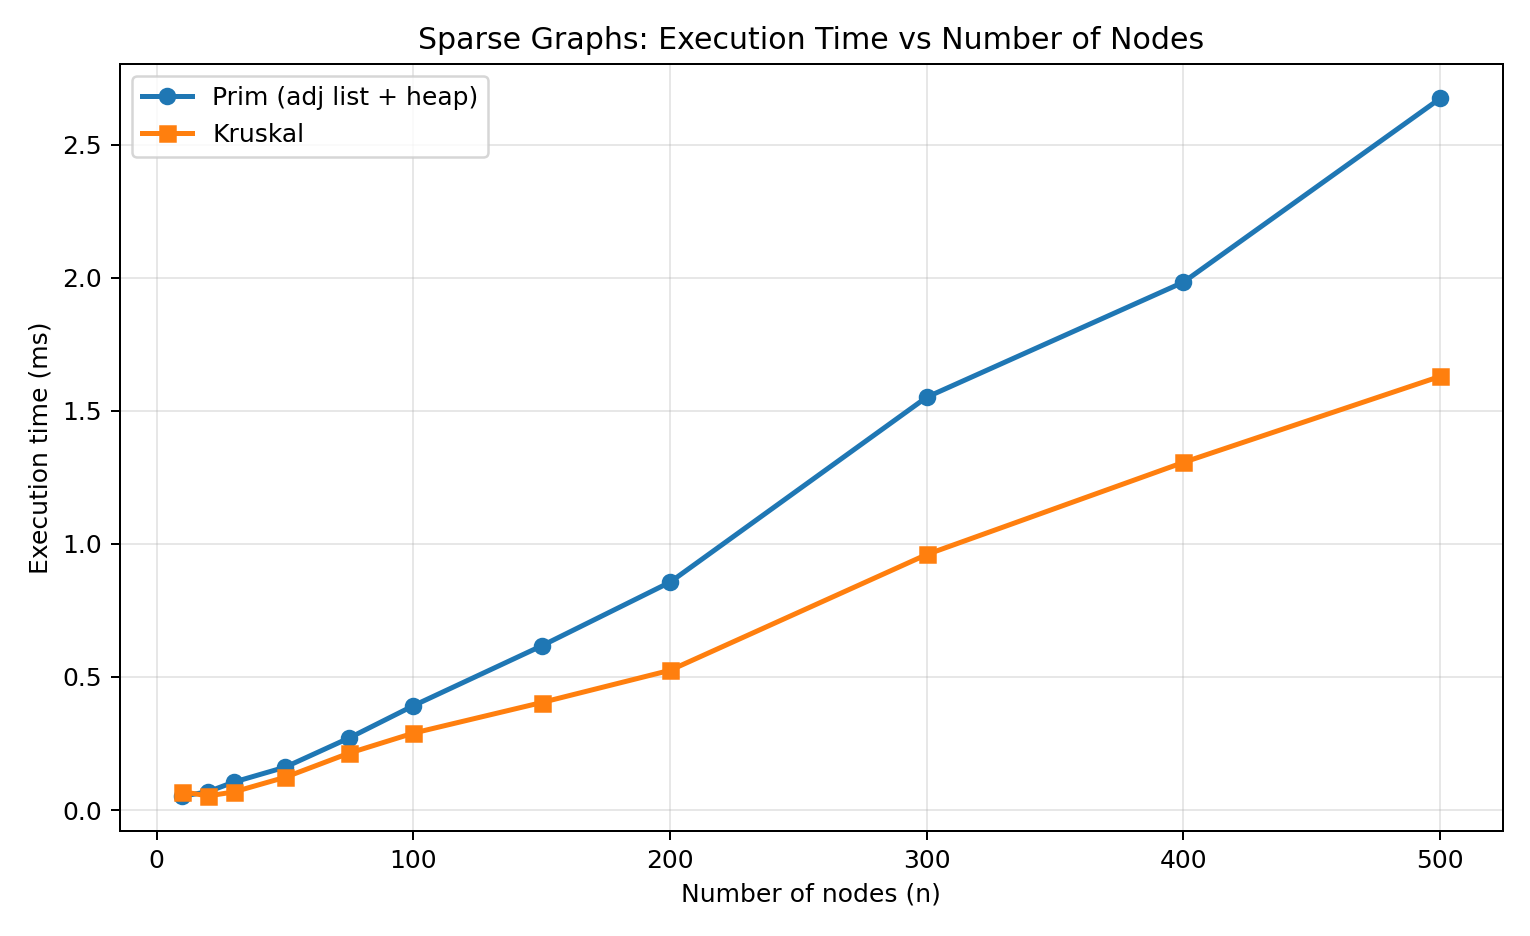
\includegraphics[width=0.88\textwidth]{figures/sparse_time_vs_nodes.png}
    \caption{Sparse graphs: execution time vs number of nodes}
    \label{fig:sparse_time_vs_nodes}
\end{figure}

Table~\ref{tab:sparse_comparison} reports runtime, memory, and operation counters for sparse graphs from $n=10$ to $n=500$ where $E \approx 2n$. Both algorithms scale smoothly, but Kruskal is faster at every tested size. At $n=100$ and $m=215$, Prim takes 0.392 ms while Kruskal takes 0.289 ms (about 1.36$\times$ faster). At $n=500$ and $m=990$, Prim reaches 2.673 ms while Kruskal is 1.629 ms (about 1.64$\times$ faster).

The counters explain this difference. Prim performs repeated heap updates and extractions, and those operations have noticeable overhead in Python. Kruskal pays one sorting cost and then executes compact union-find checks and merges, which are highly efficient. In this sparse interval, sorting up to around one thousand edges is inexpensive with Timsort, so constant factors favor Kruskal.

Memory usage remains modest for both methods in this regime. Prim's adjacency-list variant grows as $O(V+E)$, and Kruskal uses $O(E)$ for edges plus $O(V)$ for union-find. Thus, runtime is the dominant differentiator here.

\subsection{Dense Graphs: Results and Analysis}

\begin{table}[H]
    \centering
    \small
    \begin{tabular}{|c|c|c|c|c|c|}
    \hline
    \textbf{n} & \textbf{m} & \textbf{Prim Heap} & \textbf{Prim Matrix} & \textbf{Kruskal} & \textbf{Best} \\
    \hline
     10 &    29 &   0.054 &   0.051 &   0.040 & K \\
     20 &   137 &   0.159 &   0.138 &   0.063 & K \\
     30 &   265 &   0.351 &   0.337 &   0.079 & K \\
     50 &   798 &   1.398 &   0.922 &   0.213 & K \\
     75 &  1825 &   3.411 &   2.082 &   0.419 & K \\
    100 &  3171 &   6.073 &   3.697 &   0.630 & K \\
    150 &  7220 &  14.904 &   8.309 &   1.284 & K \\
    200 & 12918 &  29.667 &  18.521 &   2.335 & K \\
    250 & 20363 &  45.649 &  23.078 &   3.660 & K \\
    300 & 29117 &  65.696 &  39.036 &   4.550 & K \\
    350 & 39858 &  95.172 &  59.305 &   6.914 & K \\
    \hline
    \end{tabular}
    \caption{Dense Graphs: Algorithm Comparison (PH=Prim Heap, PM=Prim Matrix, K=Kruskal)}
    \label{tab:dense_comparison}
\end{table}

Figure~\ref{fig:dense_time_vs_nodes} shows dense-regime runtime trajectories from Table~\ref{tab:dense_comparison}. The most important feature is divergence rate: both Prim variants rise faster than Kruskal as $n$ grows. Matrix-based Prim is better than heap-based Prim, but both remain above Kruskal on medium and large inputs.

\begin{figure}[H]
    \centering
    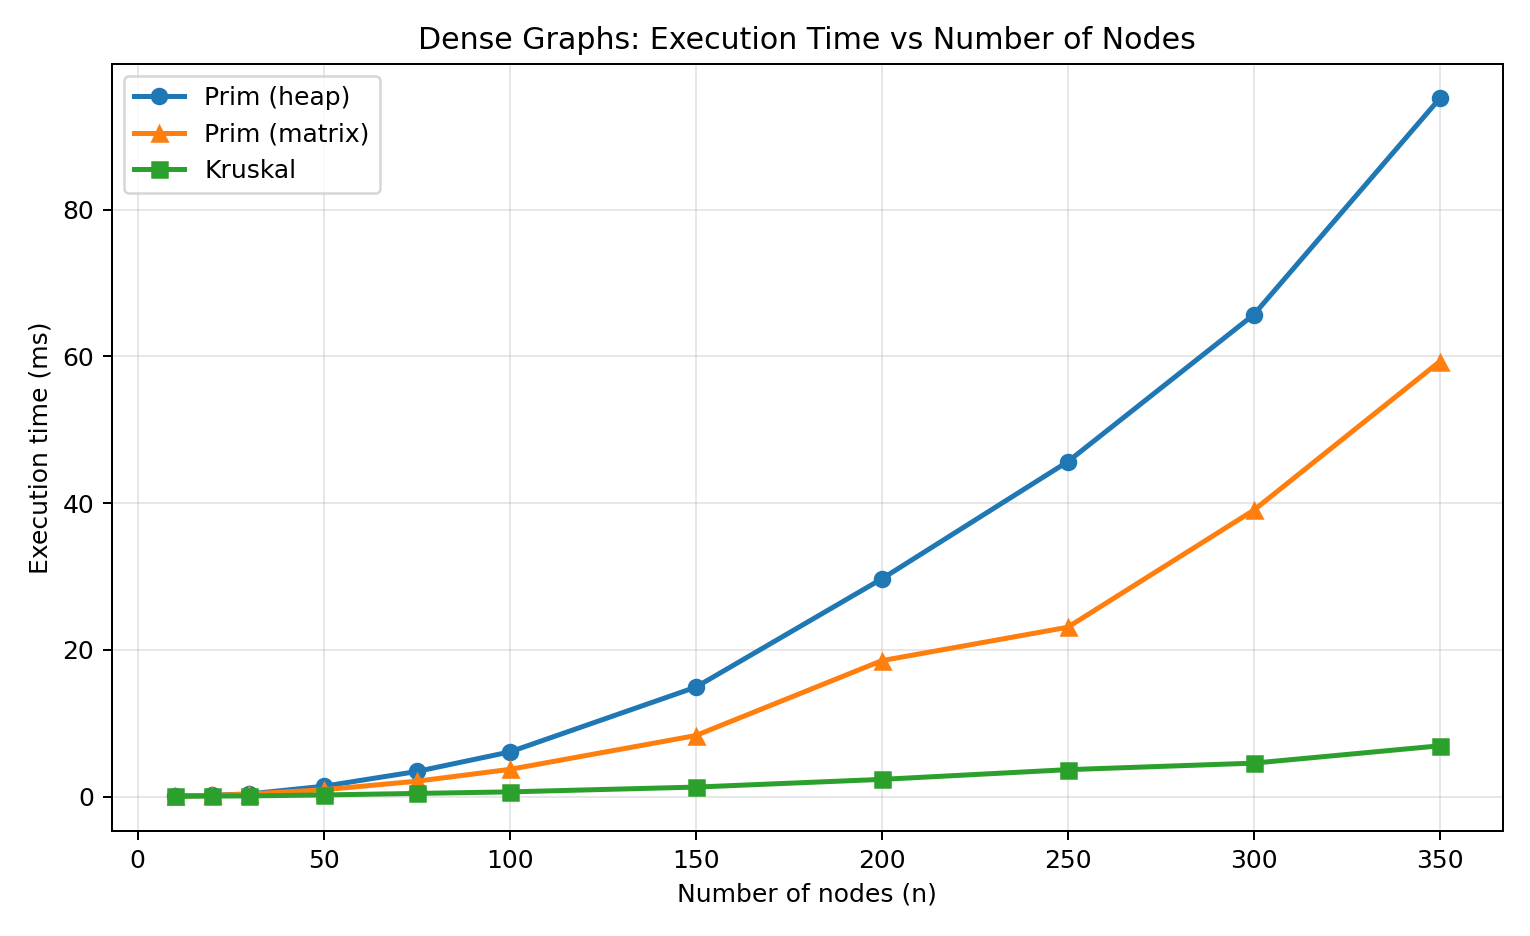
\includegraphics[width=0.88\textwidth]{figures/dense_time_vs_nodes.png}
    \caption{Dense graphs: execution time vs number of nodes}
    \label{fig:dense_time_vs_nodes}
\end{figure}

Table~\ref{tab:dense_comparison} compares Prim (heap), Prim (matrix), and Kruskal when edge counts scale quadratically. At $n=100$ and $m=3171$, Kruskal takes 0.630 ms versus 3.697 ms (Prim matrix) and 6.073 ms (Prim heap). At $n=350$ and $m=39858$, Kruskal is 6.91 ms, while Prim matrix and Prim heap reach 59.31 ms and 95.17 ms.

Two conclusions follow. First, replacing heap-based Prim with matrix-based Prim improves dense performance, confirming that reducing priority-queue overhead helps when many candidate edges exist. Second, even optimized Prim remains slower than Kruskal in this implementation. Kruskal benefits from efficient sorting and lightweight disjoint-set operations, while Prim still performs repeated global selection work over large structures.

Memory data also shows a dense-case limitation for matrix Prim: $O(V^2)$ storage grows rapidly and can become restrictive beyond moderate sizes. Kruskal stores an $O(E)$ edge list plus compact $O(V)$ union-find metadata, which remains practical in this benchmark.

\subsection{Complexity Verification}

\begin{table}[H]
    \centering
    \small
    \begin{tabular}{|l|l|c|c|}
    \hline
    \textbf{Regime} & \textbf{Algorithm} & \textbf{Log-Log Slope} & \textbf{Theoretical} \\
    \hline
        Sparse & Prim (adj list) & 1.07 & $O(V \log V) \approx 1.0$ \\
        Sparse & Kruskal & 0.94 & $O(V \log V) \approx 1.0$ \\
        Dense & Prim (heap) & 2.17 & $O(V^2 \log V) \approx 2.0$ \\
        Dense & Kruskal & 1.54 & $O(V^2 \log V) \approx 2.0$ \\
    \hline
    \end{tabular}
    \caption{Log-Log Slopes for Complexity Analysis}
    \label{tab:complexity}
\end{table}

Figure~\ref{fig:sparse_dense_comparison} combines sparse and dense curves using a logarithmic vertical axis so all trends remain visible despite different magnitudes. Dense runs are consistently above sparse runs for each algorithm, and Kruskal remains below Prim as size grows.

\begin{figure}[H]
    \centering
    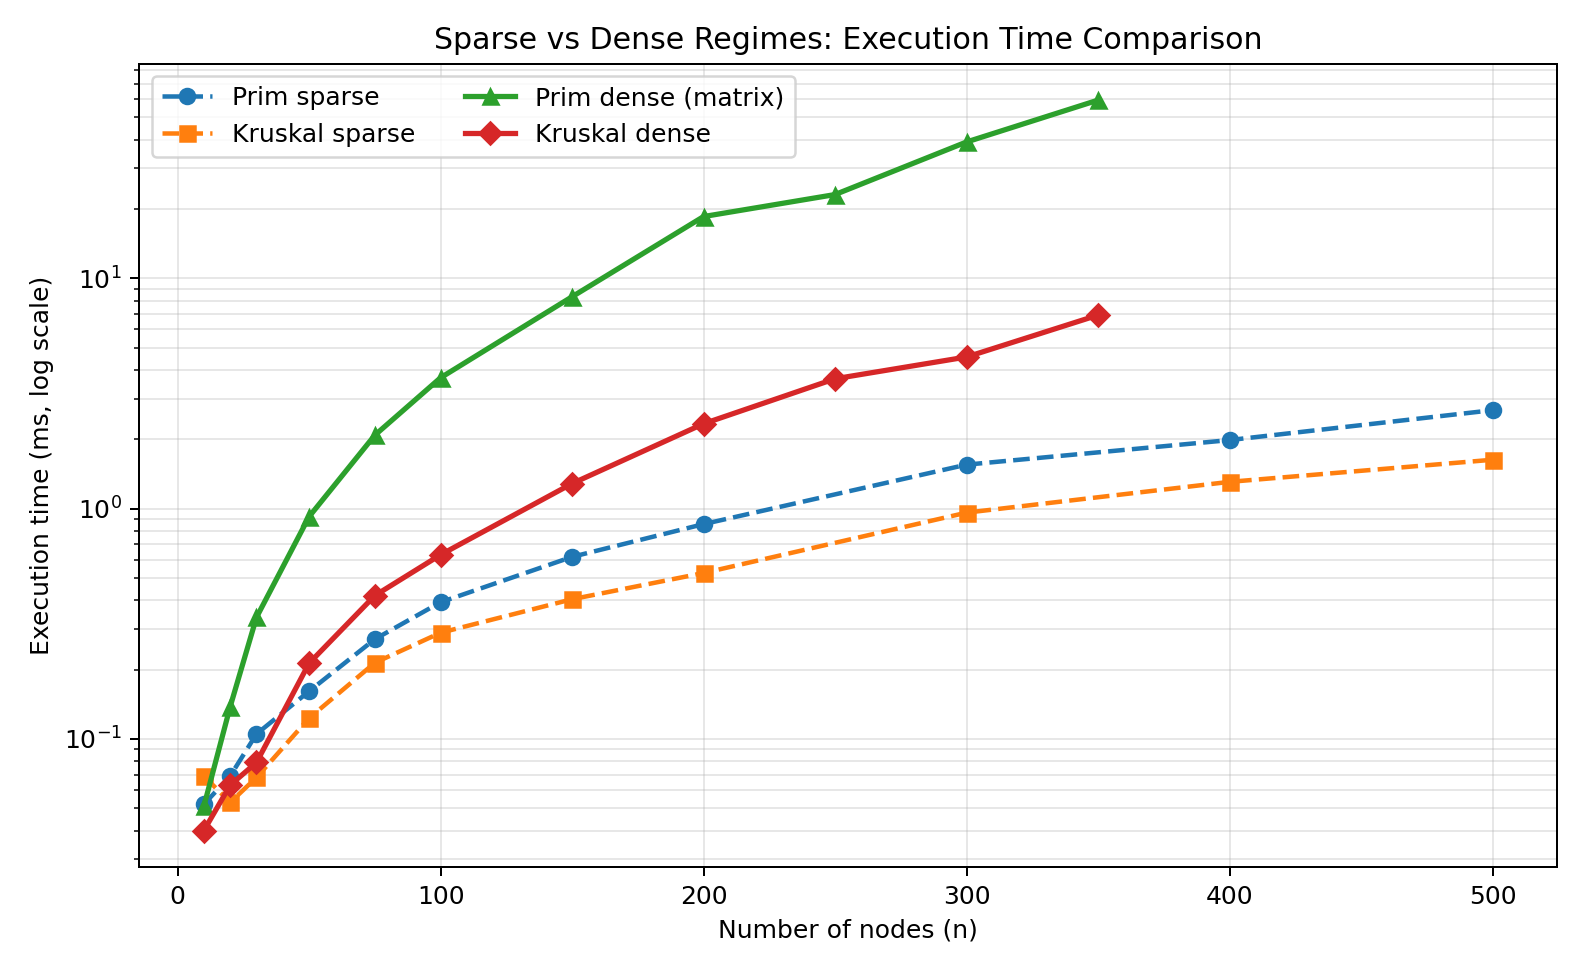
\includegraphics[width=0.90\textwidth]{figures/sparse_vs_dense_comparison.png}
    \caption{Sparse vs dense regimes: execution time comparison (log scale)}
    \label{fig:sparse_dense_comparison}
\end{figure}

Table~\ref{tab:complexity} links measured slopes to theoretical growth. In sparse mode, Prim's slope (1.07) and Kruskal's slope (0.94) indicate near-linear growth with mild logarithmic effects. In dense mode, Prim heap reaches slope 2.17, while Kruskal stays around 1.54 over the tested range.

These values show that asymptotic classes describe long-term direction, but practical ranking at laboratory scales is strongly influenced by constants and implementation details. Across all result tables, the same pattern appears: Kruskal is faster in this environment.

\section{Conclusion}

The experimental data shows that Kruskal is the better default in this laboratory for both sparse and dense graphs, and its advantage increases with size. On sparse graphs, Kruskal is typically about 35\%--65\% faster. On dense graphs, the gap is much larger, with Kruskal outperforming Prim variants by roughly 5.8$\times$ to 13.8$\times$ at larger inputs.

The comparison clarifies algorithm trade-offs. Prim offers local growth logic and can be adapted with either heap or matrix strategies, but in this Python implementation it pays higher repeated-operation overhead. Kruskal benefits from a simple execution path: one efficient sort and fast union-find checks. Its limitation is the need to handle a full global edge list, which can become memory-heavy on very large dense instances beyond this benchmark.

For practical selection in this setting: both algorithms are fast on very small inputs, but Kruskal is usually still ahead; for medium and large sparse graphs, Kruskal keeps a stable advantage; for medium and large dense graphs, Kruskal is decisively faster, while matrix Prim is the better Prim variant but still behind.

This study is limited to random undirected weighted graphs and Python runtime behavior. Different graph families, weight distributions, or lower-level implementations may alter constants. Even so, the measured trend is consistent: in the tested environment, practical algorithm choice should be guided by empirical behavior, and Kruskal is generally preferable.

\newpage

\section{Annex}

GitHub Repository: \url{https://github.com/Lucariowu/aalabs/tree/main/Lab5}
\end{document}
